% =====================================================================
%  Model-overview figure (graphical abstract style), 4 panels (a)-(d)
%  Mirrors Zhang et al. (2026) Fig 1: setup -> payoffs -> mechanism -> outcome
%
%  PREAMBLE REQUIREMENTS (put once in your main file):
%    \usepackage{tikz,amsmath,subcaption}
%    \usetikzlibrary{arrows.meta,calc,positioning}
%
%  Tip: tune the colours to your house palette; these are neutral defaults.
% =====================================================================
\definecolor{conserveC}{HTML}{1D9E75} % teal  = sustainable / cooperate
\definecolor{grabC}{HTML}{D85A30}     % coral = the payoff cut (mechanism)
\definecolor{inertC}{HTML}{888780}    % gray  = inert structure

\begin{figure}[t]
\centering

% ---------- (a) Setup: chain + threshold ----------------------------
\begin{subfigure}[t]{0.48\textwidth}
\centering
\begin{tikzpicture}[every node/.style={font=\small},>=Stealth]
  % generational chain
  \foreach \i in {0,1,2,3}{
    \node[circle,draw=inertC,minimum size=6mm] (G\i) at (\i*1.15,1.4){};
  }
  \foreach \i [evaluate=\i as \j using int(\i+1)] in {0,1,2}{
    \draw[->,inertC] (G\i) -- (G\j);
  }
  \node[font=\scriptsize,inertC] at (0,1.78){$G_t$};
  % threshold regeneration glyph
  \draw[inertC,thick] (0,0.05) -- (1.6,0.05) -- (1.6,-0.45) -- (3.45,-0.45);
  \node[font=\scriptsize] at (1.6,-0.7){$\tau$};
  \node[font=\scriptsize,inertC,anchor=west] at (0,-1.05)
        {$x\le\tau$ persists, $x>\tau$ collapses};
\end{tikzpicture}
\caption{Infinite chain; threshold regeneration.}
\label{fig:model-a}
\end{subfigure}
\hfill
% ---------- (b) Payoffs: PD vs stag hunt ----------------------------
\begin{subfigure}[t]{0.48\textwidth}
\centering
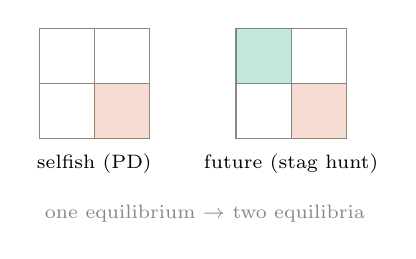
\begin{tikzpicture}[font=\scriptsize]
  % PD matrix
  \draw[inertC] (0,0) rectangle (1.4,1.4);
  \draw[inertC] (0.7,0)--(0.7,1.4)  (0,0.7)--(1.4,0.7);
  \fill[grabC,opacity=0.22] (0.7,0) rectangle (1.4,0.7); % sole eq: collapse
  \node at (0.7,-0.32){selfish (PD)};
  % Stag-hunt matrix
  \begin{scope}[xshift=2.5cm]
    \draw[inertC] (0,0) rectangle (1.4,1.4);
    \draw[inertC] (0.7,0)--(0.7,1.4)  (0,0.7)--(1.4,0.7);
    \fill[conserveC,opacity=0.25] (0,0.7) rectangle (0.7,1.4); % sustain eq
    \fill[grabC,opacity=0.22] (0.7,0) rectangle (1.4,0.7);     % collapse eq
    \node at (0.7,-0.32){future (stag hunt)};
  \end{scope}
  \node[anchor=west,inertC] at (-0.05,-0.95)
        {one equilibrium $\to$ two equilibria};
\end{tikzpicture}
\caption{Valuing the future turns PD into a stag hunt.}
\label{fig:model-b}
\end{subfigure}

\vspace{0.9em}

% ---------- (c) Mechanism: accountability slides delta* -------------
\begin{subfigure}[t]{0.48\textwidth}
\centering
\begin{tikzpicture}[>=Stealth,font=\scriptsize]
  \draw[inertC] (0,0) -- (0,2.0);            % payoff axis
  \draw[inertC] (0,0) -- (3.3,0);            % delta axis
  \node[anchor=north] at (3.3,0){$\delta$};
  % grab line K (solid) and K-c (dashed, lower)
  \draw[inertC,thick] (0,1.45) -- (3.1,1.45);
  \node[anchor=west] at (3.12,1.45){$K$};
  \draw[grabC,thick,dashed] (0,0.85) -- (3.1,0.85);
  \node[anchor=west,grabC] at (3.12,0.85){$K\!-\!c$};
  \draw[->,grabC] (0.55,1.43) -- (0.55,0.9); % the drop
  % conserve line tau/(1-delta) rising
  \draw[conserveC,very thick] (0,0.18) .. controls (1.8,0.7) .. (3.0,2.0);
  \node[anchor=south,conserveC] at (2.7,1.85){conserve};
  % crossings
  \fill[inertC] (2.05,1.45) circle (1.6pt);
  \fill[grabC]  (1.25,0.85) circle (1.6pt);
  \draw[->,grabC] (1.95,-0.32) -- (1.2,-0.32);
  \node[anchor=north] at (2.05,-0.3){$\delta^\star$};
  \node[anchor=north,grabC] at (1.05,-0.3){$\delta^\star\!(c)$};
\end{tikzpicture}
\caption{Accountability drops the grab payoff, sliding $\delta^\star$ left.}
\label{fig:model-c}
\end{subfigure}
\hfill
% ---------- (d) Outcome: 41% -> 86% --------------------------------
\begin{subfigure}[t]{0.48\textwidth}
\centering
\begin{tikzpicture}[>=Stealth,font=\scriptsize]
  \draw[inertC] (0,0) -- (3.3,0);
  \fill[inertC,opacity=0.55] (0.6,0) rectangle (1.3,0.82);   % 41%
  \fill[conserveC] (2.0,0) rectangle (2.7,1.72);             % 86%
  \node[anchor=south] at (0.95,0.82){41\%};
  \node[anchor=south,conserveC] at (2.35,1.72){86\%};
  \node[anchor=north] at (0.95,0){baseline};
  \node[anchor=north] at (2.35,0){+\,account.};
  \draw[->,grabC,thick] (1.35,0.95) .. controls (1.7,1.6) .. (1.95,1.55);
\end{tikzpicture}
\caption{Conservation rises from baseline to the accountable level.}
\label{fig:model-d}
\end{subfigure}

\caption{\textbf{The model in one figure.}
(a) The intergenerational good is an infinite chain with threshold
regeneration at $\tau$: take at most $\tau$ and the pool persists,
take more and it collapses irreversibly.
(b) Once the future is weighted, the stage game shifts from a
prisoner's dilemma (a single collapse equilibrium) to a stag hunt
(a payoff-dominant sustainable equilibrium alongside a risk-dominant
collapse equilibrium).
(c) An accountability cost $c$ lowers the grab payoff from $K$ to
$K-c$, sliding the selection threshold $\delta^\star(c)=1-\tau/(K-c)$
to the left.
(d) The net effect on the conserving share, calibrated to the
baseline rate.}
\label{fig:model-overview}
\end{figure}
